% For VIM to recognize the document syntax \begin{document} and \end{document}
% - However, the compilation will fail!! So don't forget to comment the
%   directives before compiling!!'
%
%\begin{document}
%
% CHAPTER - Introduction -------------------------
\chapter{Introduction}%
\label{ch:introduction}

\section{Problem statement}
\label{sec:prob-stat}
    Design a remote control with three buttons that can
remotely control the television (TV). It should be very
light, powered by batteries and controls your TV via an
infrared emitter. The TV has a built-in infrared receiver. A
button on the remote control switches the TV on/off and
will be labeled with the word "Power". The other two
buttons are used to scroll up/down and select the available
channels and they are labeled with the arrows up/down.

\section{Market research}
\label{sec:market-research}
	A TV remote is a device which is used to operate a television from distance in a wirelessly mode. It also makes the TV usage more simpler, making it more user friendly with its suggestive buttons. These buttons control functions such as power, volume, channel switch and various other features.

TV remotes are composed by the TV remote Shell,
the TV remote membrane, one LED and a data acquisition \& Infrared emitter PCB.

The unit cost of universal TV Remotes is about 3 to 5 euros.

As we can see through this next graphic, the amount of televisions sold per year is about 200 million per year, with a tendency to increase for bigger numbers over the next years. This also means that it is needed a tv remote for each television or can also happen the case which a tv remote that came with the TV stopped working, which leads for a need to buy another remote.

\begin{figure}
\centering
    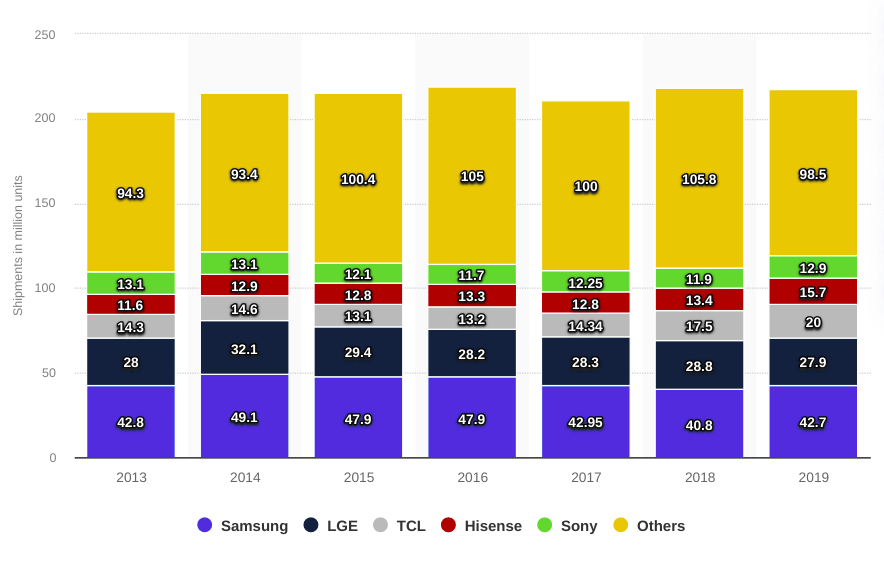
\includegraphics[width=0.9\columnwidth]{./img/tvsellings.png}
  \caption{Global LCD TV unit shipments from 2015 to 2019, by vendor (in millions)* from~\cite{tvsellings})}%
\label{fig:tvsells}
\end{figure}
%
%%% Local Variables:
%%% mode: latex
%%% TeX-master: "../../dissertation"
%%% End:
